\documentclass[FIPLY_base.tex]{subfiles}

%\author{Andreas Denkmayr}
%\date{19. Februar 2016}

\begin{document}
\subsection{Musik}
[Android Developers \cite{adMediaPlayer}, \citeauthor{bMediaPlayer} \cite{bMediaPlayer}]

\subsubsection{Lokalisierung der Musikdateien}
Am Beginn der Arbeit wurde der Music-Ordner nach mp3-Files durchsucht.
\begin{lstlisting}
File home = new File(Environment.getExternalStorageDirectory()
	.getAbsolutePath() + "/Music";);
songs = new ArrayList<>();
if (home.listFiles(new FileExtensionFilter()) != null) {
	for (File file : home.listFiles(new FileExtensionFilter())) {
		HashMap<String, String> song = new HashMap<>();
		song.put("songTitle", file.getName());
		song.put("songPath", file.getPath());
		songs.add(song);
	}
}    
\end{lstlisting}

\ \\
Im Laufe der Entwicklung stellte sich heraus, dass jeder Benutzer seine Musikdateien in einem anderen Ordner und in verschiedenen Dateiformaten abspeichert. 
Die Lösung für dieses Problem stellt der Android Mediastore dar. 
Über diesen können Abfragen nach verschiedenen Medientypen z.B.: Musik, Fotos oder Videos durchgeführt werden. Von diesen Medientypen können Name, Pfad, Dateigröße und vieles mehr ausgelesen werden.
  
\ \\  
Die Datenabfrage gegenüber dem Mediastore erfolgt über einen ContentResolver mit Hilfe der query()-Methode.
\begin{lstlisting}
public final @Nullable Cursor query(@NonNull Uri uri, @Nullable String[] projection, @Nullable String selection, @Nullable String[] selectionArgs, @Nullable String sortOrder) {
	return query(uri, projection, selection, selectionArgs, sortOrder, null);
}
\end{lstlisting}

\ \\
Für den Musicplayer benötigen wir alle Audiodateien, die Musik beinhalten.
\begin{lstlisting}
ContentResolver cr = context.getApplicationContext()
	.getContentResolver();
Uri uri = MediaStore.Audio.Media.EXTERNAL_CONTENT_URI;
String selection = MediaStore.Audio.Media.IS_MUSIC + "!= 0";
String sortOrder = MediaStore.Audio.Media.TITLE_KEY + " ASC";
Cursor cur = cr.query(uri, null, selection, null, sortOrder);
\end{lstlisting}

\newpage
\ \\
Für jede Zeile im Cursor cur wird eine HashMap aus 2 Strings erstellt die den Titel und den Pfad eines Songs beinhaltet. Diese HashMaps werden anschließend zu einer ArrayList hinzugefügt.
\begin{lstlisting}
songs = new ArrayList<>();
HashMap<String, String> song = new HashMap<>();
while(cur.moveToNext())
{
	song.put("songTitle", cur.getString(cur
		.getColumnIndex(MediaStore.Audio.Media.TITLE)));
	song.put("songPath", cur.getString(cur
		.getColumnIndex(MediaStore.Audio.Media.DATA)));
	songs.add(song);
}
\end{lstlisting}




\subsubsection {Verwalten von Playlists}
\begin{figure}[H]
	\begin{subfigure}[b]{0.3\textwidth}
	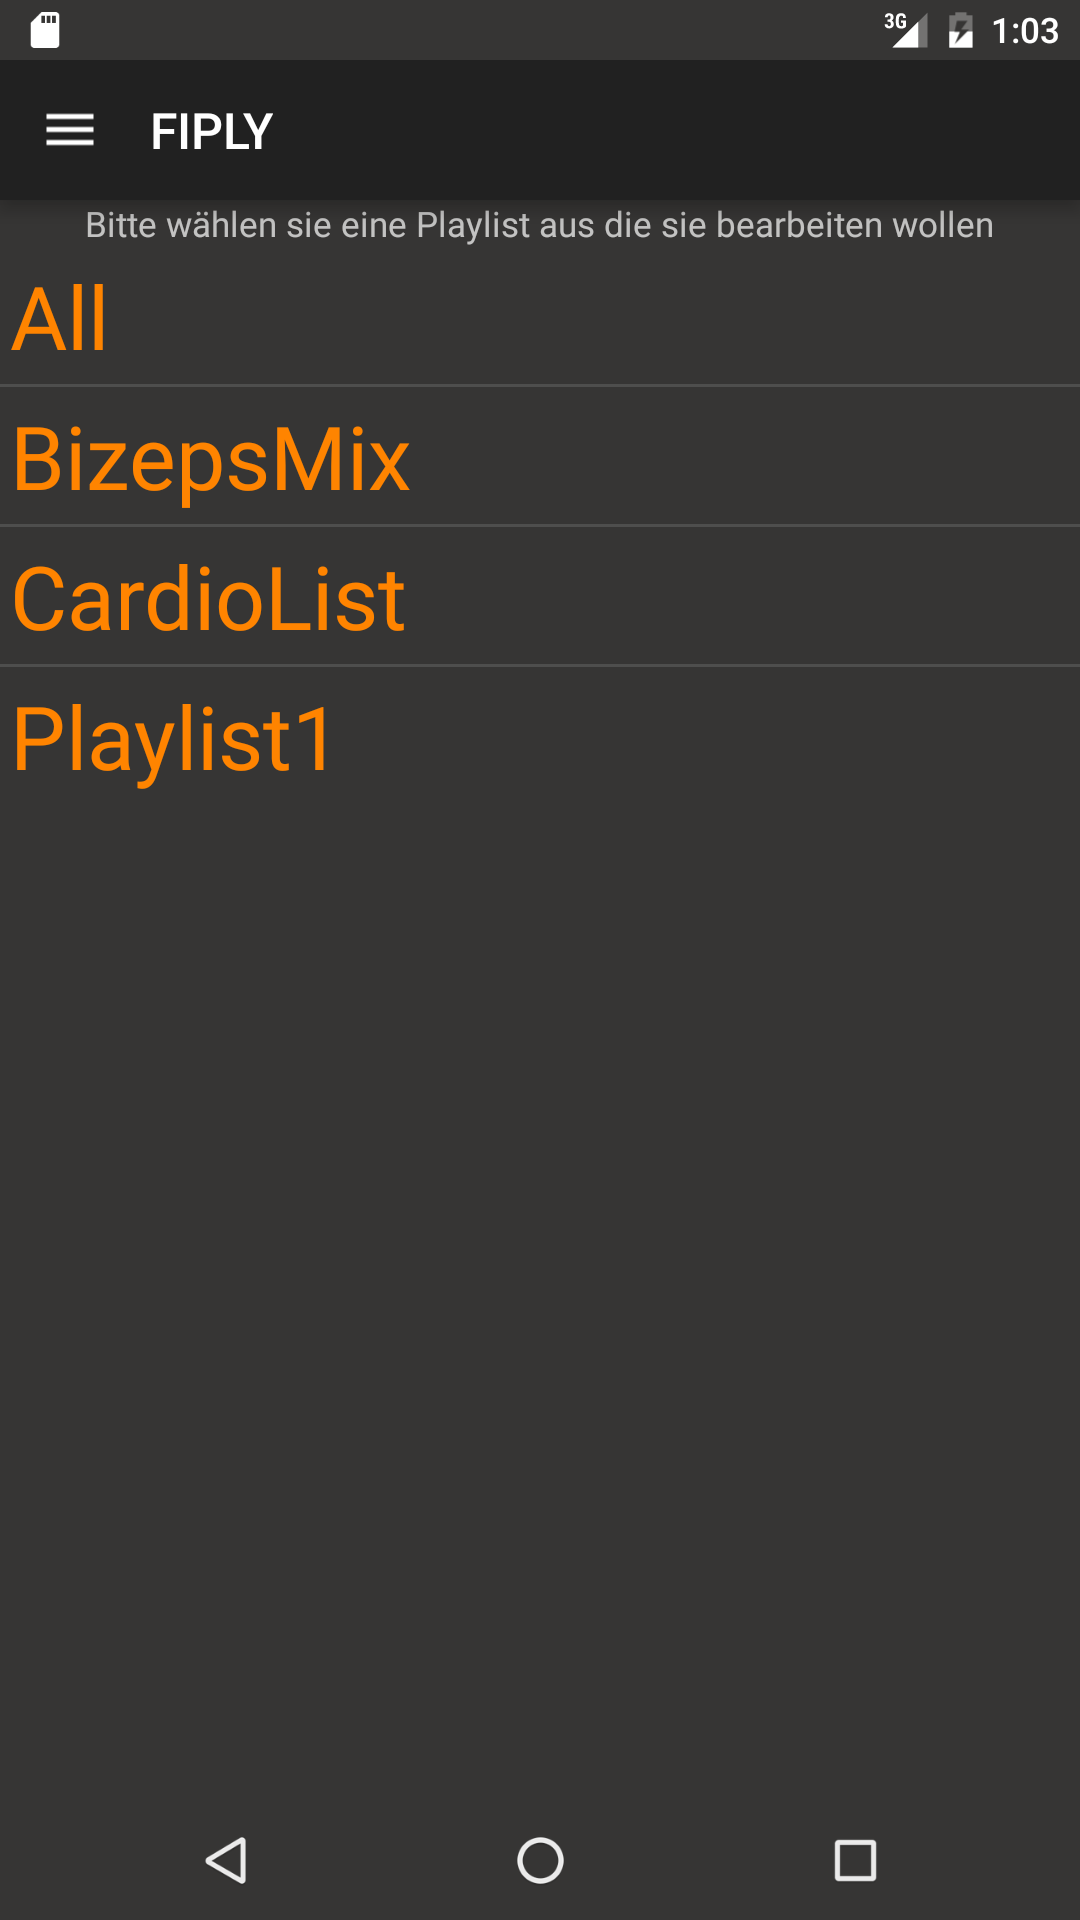
\includegraphics[scale=0.15]{img/musicPlaylistView1}
	\end{subfigure}
	\hfil
	\begin{subfigure}[b]{0.3\textwidth}
	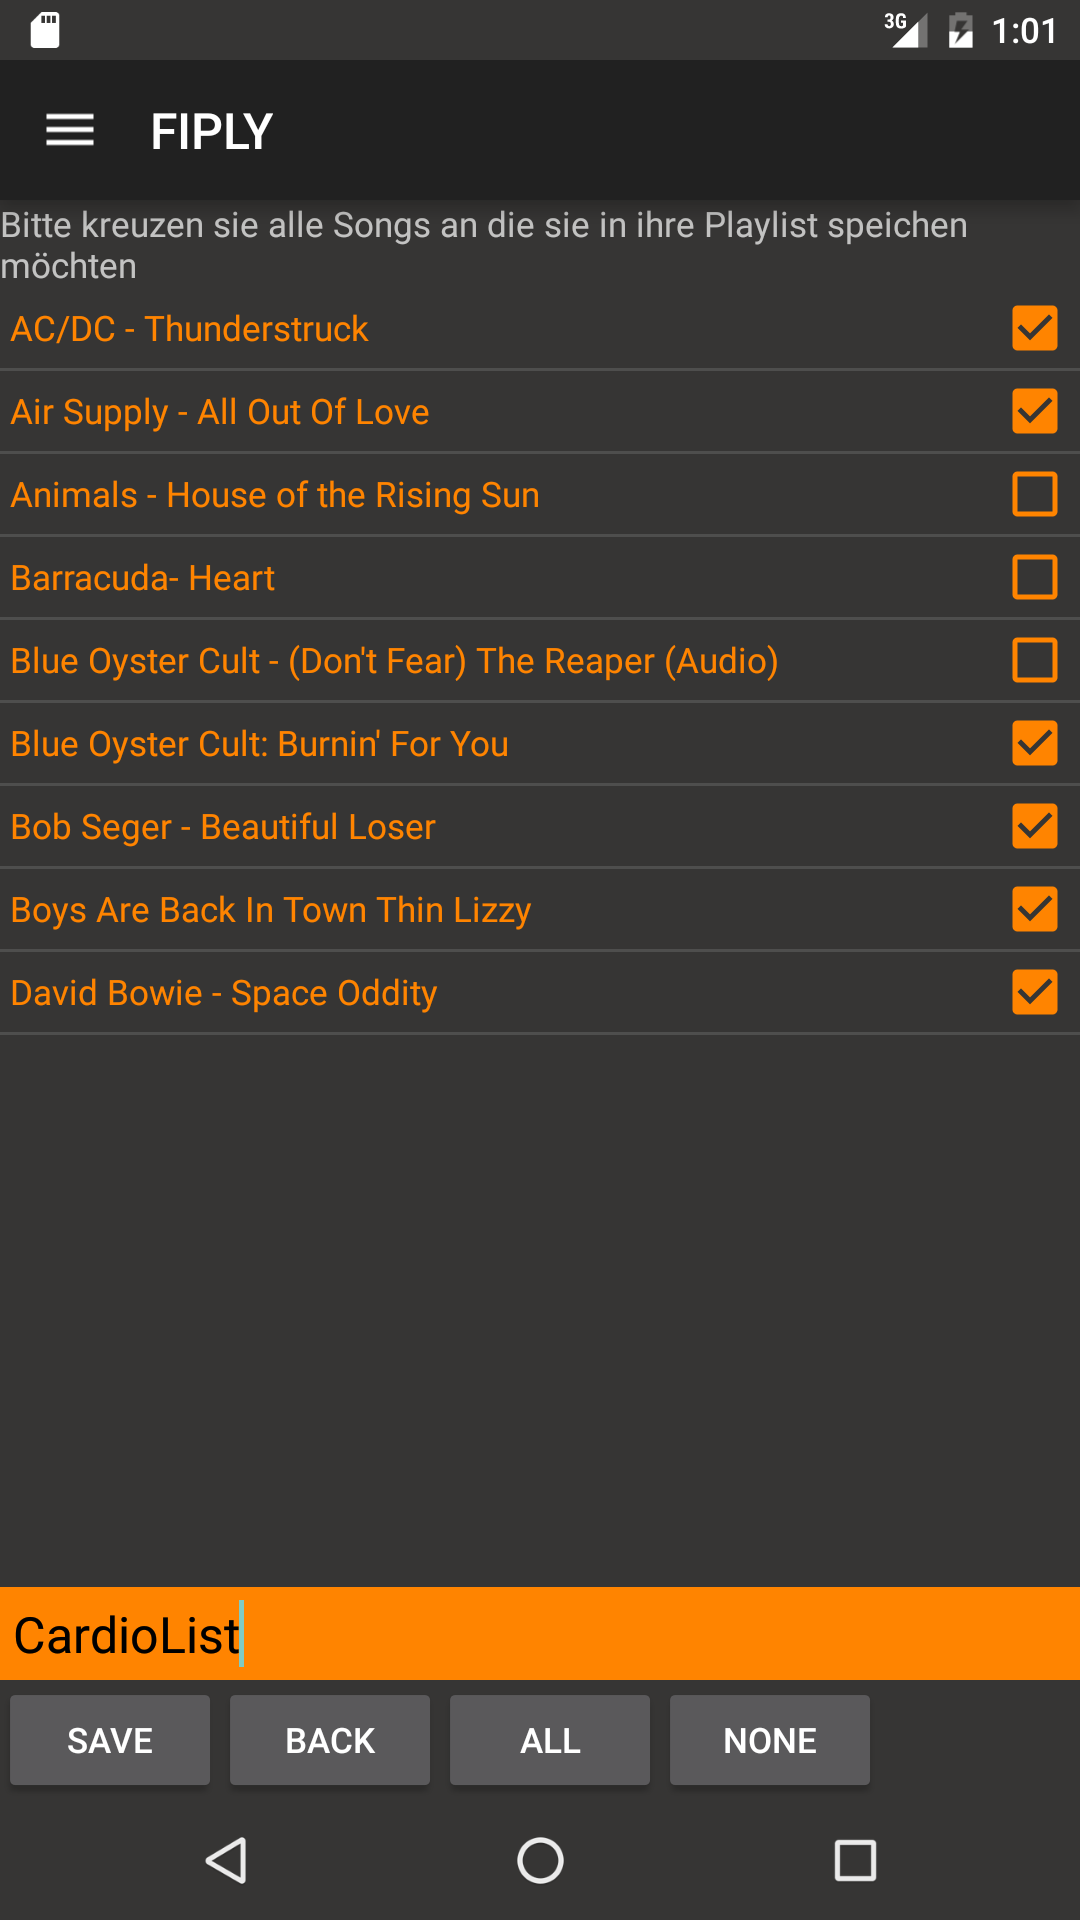
\includegraphics[scale=0.15]{img/musicSongView1}
	\end{subfigure}
	\caption{Bei Klicken eines Elements in Screenshot 1 werden alle Songs angezeigt (Screenshot 2). 
	Mittels der Checkboxenty werden jene Songs markiert, die sich in der ausgewählten Playlist befinden.}
\end{figure}

\ \\
Im ersten Screenshot sieht man die Auswahl der erstellten Playlists, wobei die Playlist ''All' nicht bearbeitet werden kann und alle eingelesenen Songs darstellt.
Zusätzlich zu der ''All''-Playlist kann der Benutzer eigene Playlists anlegen und diese auch bearbeiten.

\ \\
Der All und der None Button helfen dem Benutzer schnell alle Songs zu markieren oder die Markierung aller Elemente aufzuheben.

\ \\
Der Back Button führt zurück zur Playlistauswahl und verwirft alle nicht gespeicherten Änderungen an der aktuellen Playlist.

\ \\
Wird der Save-Button gedrückt wird für alle Positionen abgespeichert ob das Element an der jeweiligen Position markiert ist. Dies erfolgt über ein SparseBooleanArray. 
Anschließend wird eine Liste erstellt, in der nur die angekreuzten Elemente enthalten sind. Diese Liste wird als eine neue Playlist in die PlaylistSongs-Tabelle gespeichert. 
Dabei wird als Playlistname der in das EditText eingetragene Titel unter der ListView übernommen.

\begin{lstlisting}
SparseBooleanArray checked = lvSongs.getCheckedItemPositions();
for (int i = 0; i < songs.size(); i++) {
    if (checked.get(i)) {
        checkedSongs.add(songs.get(i));
    }
}
psrep.reenterPlaylist(etName.getText().toString(), checkedSongs);
\end{lstlisting}



\newpage
\subsubsection {Abspielen der Playlists.}
Das Abspielen der Songs erfolgt über den MediaPlayer (API level 1). \newline
Das Wechseln eines Songs wurde mithilfe der changeSong-Methode realisiert. \newline
Diese Methode nimmt die Playlist und den Index eines Songs in dieser Playlist entgegen, kümmert sich um das Setzen der Datenquelle für den MediaPlayer und bereitet den MediaPlayer auf die Wiedergabe vor. 
Zusätzlich wird der neue Songname angezeigt und die laufende Aktualisierung der Fortschrittsanzeigen wird durch den Aufruf von updateProgressBar() eingeschaltet. 

\begin{lstlisting}
public void changeSong(int songIndex, String playlist) {
    aktPlaylist = playlist;
    setPlaylist(psrep.getByPlaylistName(aktPlaylist));
    setSongIndex(songIndex);
    try {
        mp.reset();
        mp.setDataSource(getPlaylist().get(getSongIndex())
        	.get("songPath"));
        mp.prepare();
    } catch (IOException e) {
        e.printStackTrace();
    }
    progressBar.setProgress(0);
    updateProgressBar();
    tvSongname.setText(getPlaylist().get(getSongIndex())
    	.get("songTitle"));
    tvTotalDur.setText(millisecondsToHMS(mp.getDuration()));
}

private void updateProgressBar() {
    mHandler.postDelayed(mUpdateDurTask, 100);
}
\end{lstlisting}
Der mUpdateDurTask aktualisiert die Fortschrittsanzeigen 10 mal pro Sekunde.
Da mp.getDuration Millisekunden zurückliefert, konvertiert die \newline millisecondsToHMS-Methode die Songdauer in einen String im hh:mm:ss Format (ISO 8601).

\begin{lstlisting}
private Runnable mUpdateDurTask = new Runnable() {
    @Override
    public void run() {
        long currentDur = mp.getCurrentPosition();
        tvCurrentDur.setText(millisecondsToHMS(currentDur));
        int progress = getProgressPercentage(currentDur, mp.getDuration());
        progressBar.setProgress(progress);
        mHandler.postDelayed(this, 100);
    }
};
\end{lstlisting}

\begin{figure}[H]
	\begin{subfigure}[b]{0.3\textwidth}
	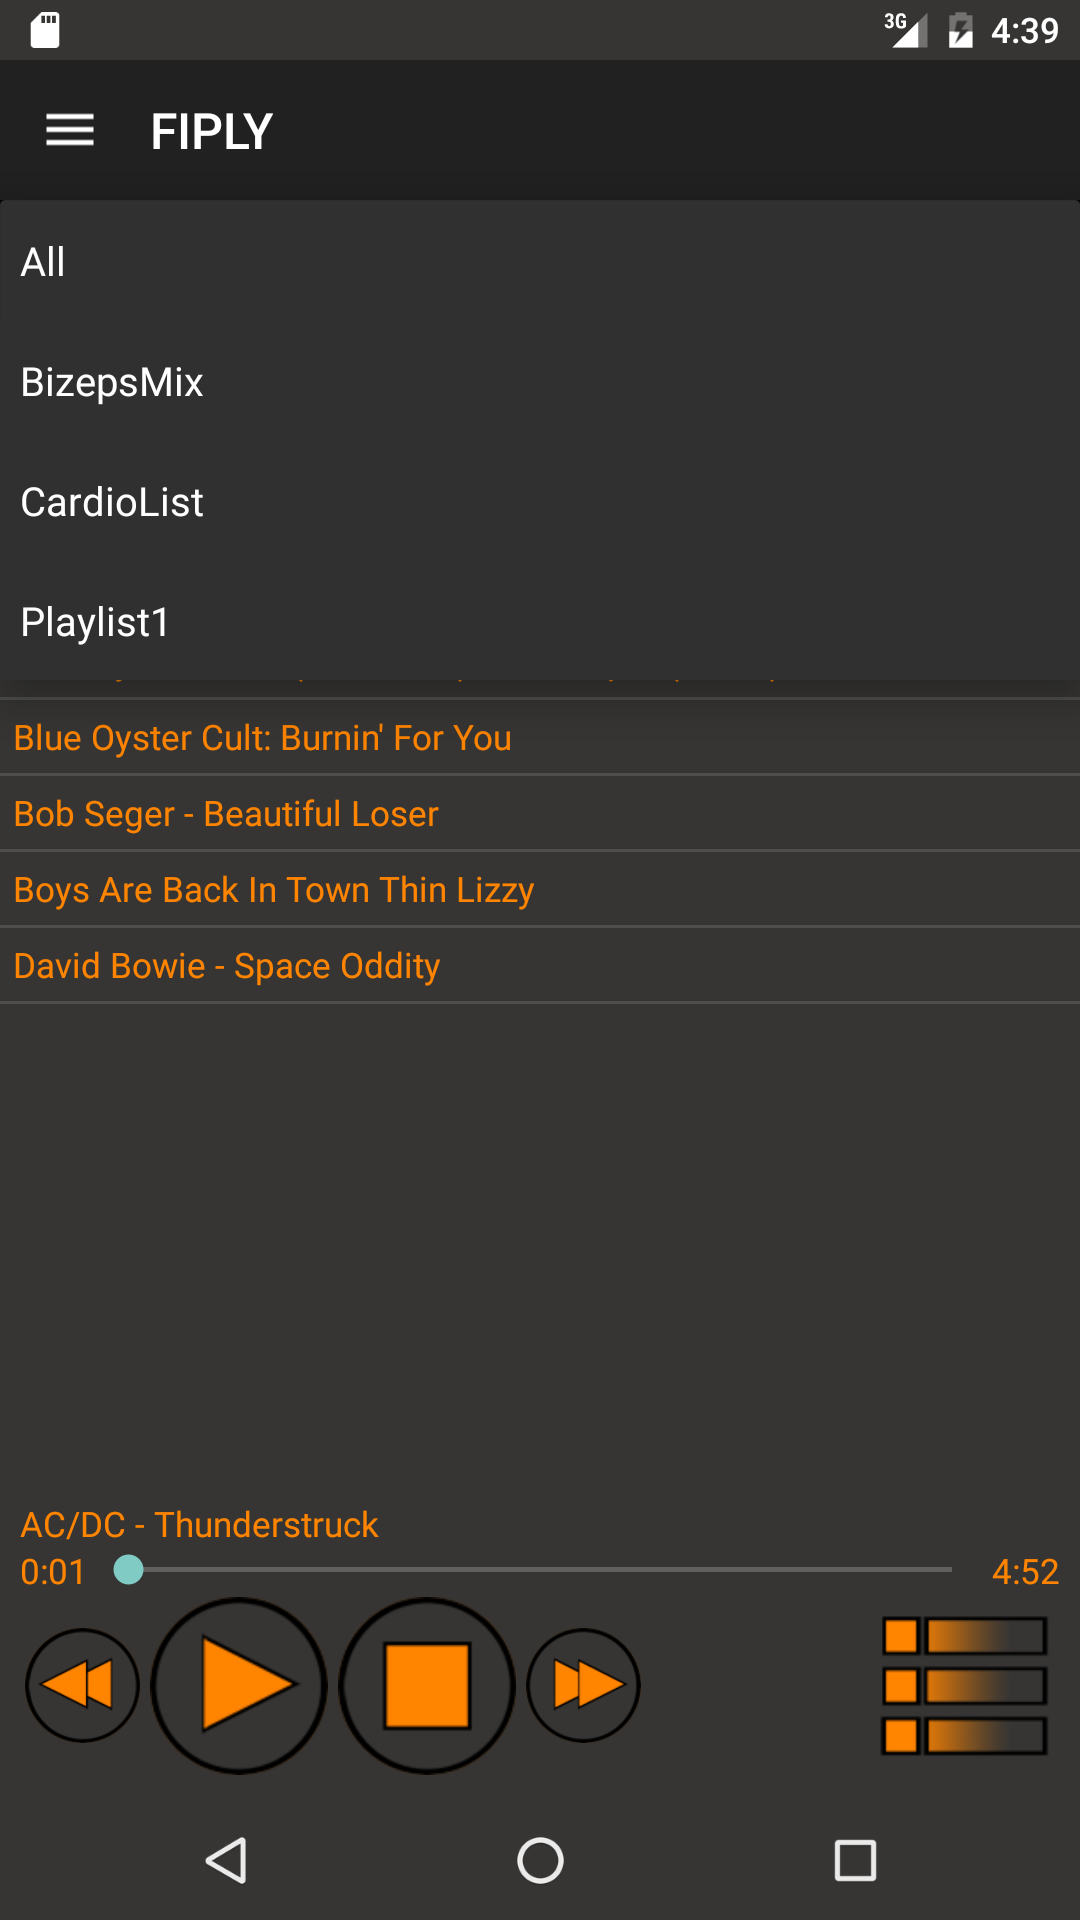
\includegraphics[scale=0.17]{img/musicListenView1}
	\end{subfigure}
	\hfil
	\begin{subfigure}[b]{0.3\textwidth}
	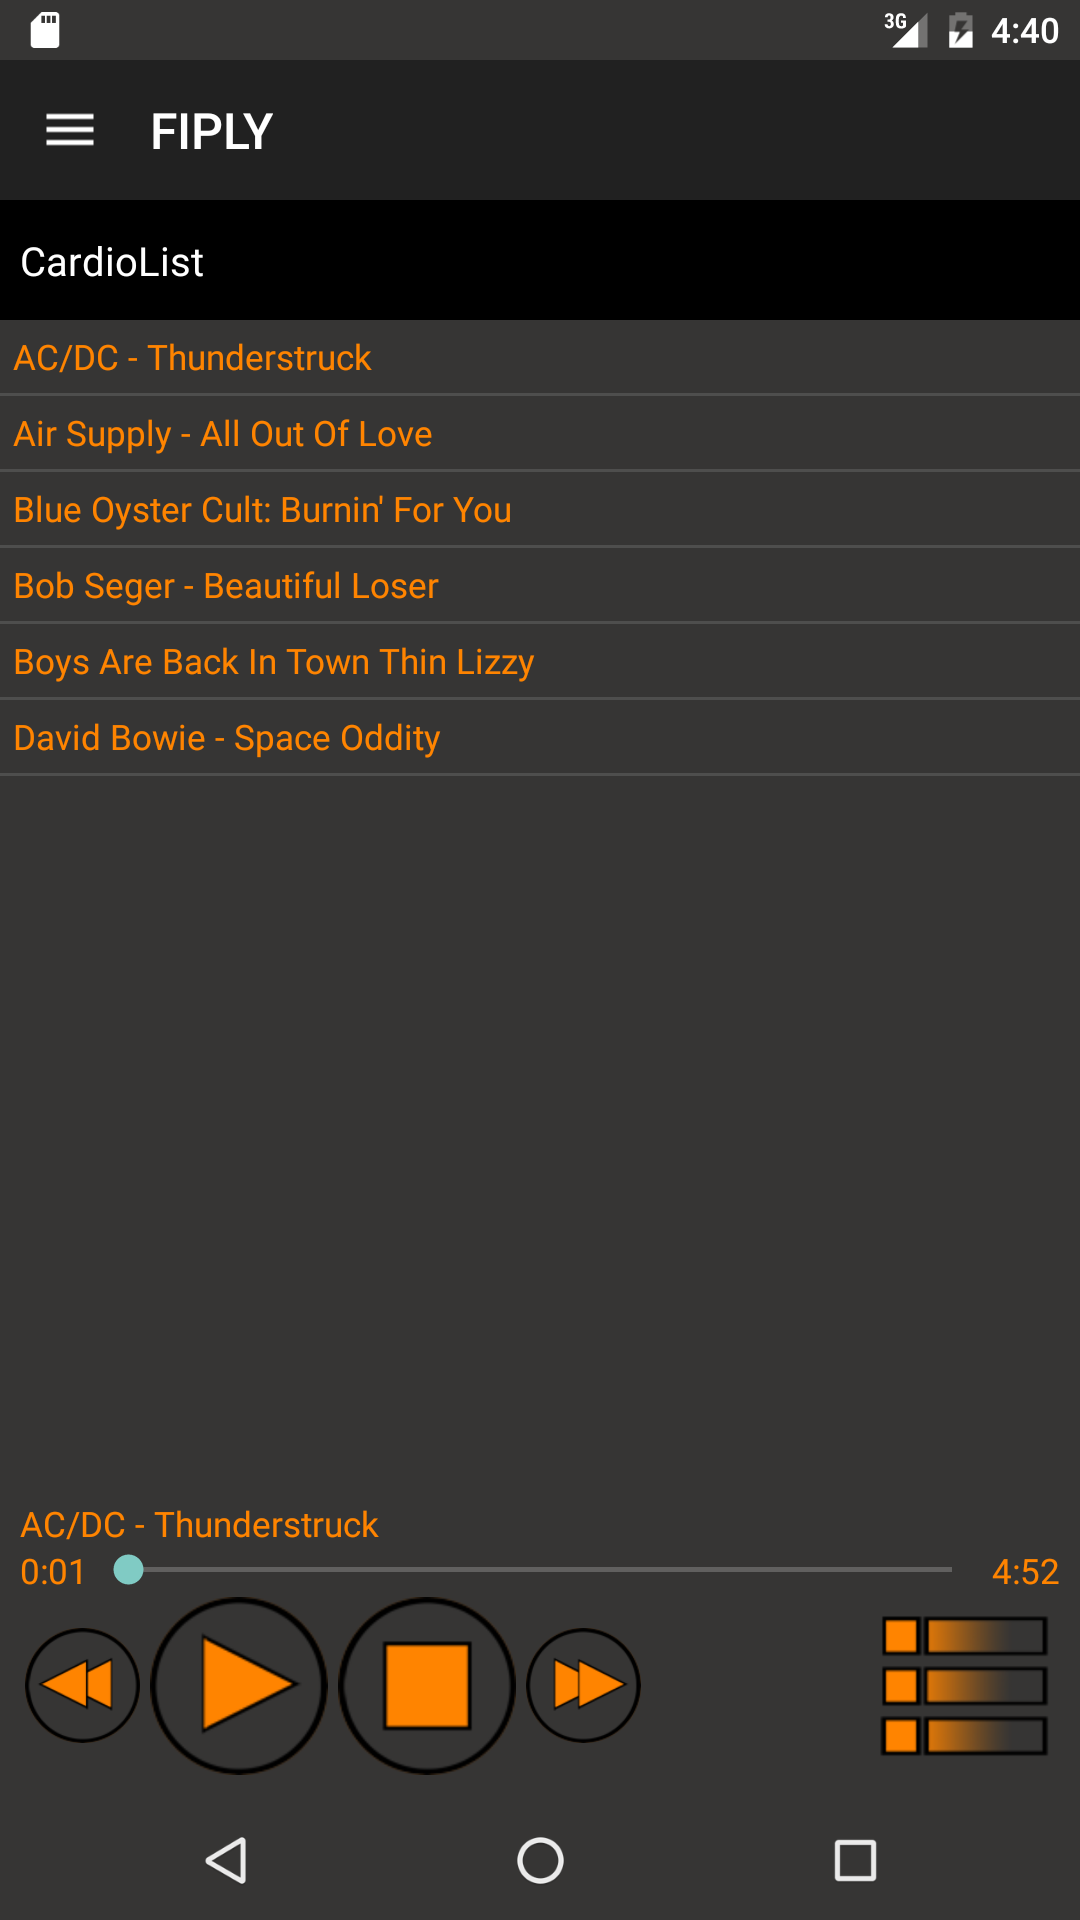
\includegraphics[scale=0.17]{img/musicListenView2}
	\end{subfigure}
	\caption{In einem Spinner kann eine Playlist ausgewählt werden. Bei Klick auf einen Song wird dieser abgespielt.}
\end{figure}

\ \\
Während der Benutzer sich in einer Traingssession befindet kann jederzeit die Musikwiedergabe gestartet werden.
Bei Klick auf den Play-Button wird die ''All''-Playlist in alphabetisch aufsteigender Reihenfolge abgespielt. \newline
Die Playlist beziehungsweise der aktuell abgespielte Song kann geändert werden, indem man durch Klick auf den Musikmodus Button in den Musikmodus gewechselt wird. \newline
In diesem Modus wird über den Spinner die Playlist gewechselt. \newline
In der aktuell ausgewählten Playlist kann man direkt zu einem bestimmten Song wechseln, indem man auf den Songtitel klickt. 
Dieser wird abgespielt und nach Ende des Songs wird sofort der nächste Playlisteintrag gestartet.

\newpage
\subsubsection {MusicControls}

\begin{figure}[H]
	\begin{subfigure}[b]{0.3\textwidth}
	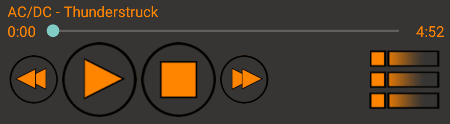
\includegraphics[scale=0.55]{img/musicControls}
	\end{subfigure}
	\hfil
	\begin{subfigure}[b]{0.3\textwidth}
	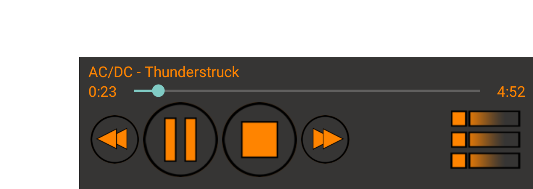
\includegraphics[scale=0.55]{img/musicControlsPlaying}
	\end{subfigure}
	\caption{Die MusicControls in Ruhe und während einer Wiedergabe.}
\end{figure}

\begin{itemize}
\item Durch den Zurück und durch den Weiter Button kann auf den vorherigen beziehungsweise auf den nächsten Song gewechselt werden. 
\item Der Play Button dient dem Starten der Musikwiedergabe. \newline
Während der Musikwiedergabe erscheint an dieser Stelle der Pause Button mit dem man die Musik pausieren kann. 
\item Der Stop Button beendet die aktuelle Wiedergabe und setzt den Wiedergabefortschritt auf den Beginn des Songs. 
\item Der Musikmodus Button befindet sich in der Ecke unten rechts. \newline
Dieser stellt den aktuellen Modus durch seine Einfärbung dar und ermöglicht einen Wechsel zwischen dem Übungsmodus und dem Musikmodus.
Im Übungsmodus wird die aktuelle Übung und die Anweisungen zum Trainieren angezeigt. \newline
Der Musikmodus hingegen ermöglicht ein Wechseln der Playlist und den manuellen Wechsel auf einen bestimmten Song. 
\item Links von der Fortschrittsleiste wird der Fortschritt des aktuellen Songs im hh:mm:ss Format (ISO 8601) angezeigt. 
\item Die Fortschrittsleiste wird durch eine SeekBar über diesen Buttons implementiert. Diese SeekBar stellt den aktuellen Fortschritt des aktuellen Songs dar. 
Bei Klicken auf oder Ziehen an der Fortschrittsleiste kann man den Fortschritt der Wiedergabe manipulieren. 
\item Rechts von der Fortschrittsleiste wird die Gesamtdauer des Songs im hh:mm:ss Format (ISO 8601) angezeigt.
\item Der Name des aktuellen Songs wird in einer TextView über den Fortschrittsanzeigen dargestellt.
\end{itemize}

\end{document}